\documentclass[UTF8]{ctexart}

% Language setting
% Replace `english' with e.g. `spanish' to change the document language
\usepackage[english]{babel}

% Set page size and margins
% Replace `letterpaper' with `a4paper' for UK/EU standard size
\usepackage[a4paper,top=2cm,bottom=2cm,left=3cm,right=3cm,marginparwidth=1.75cm]{geometry}

% Useful packages
\usepackage{amsmath}
\usepackage{graphicx}
\usepackage[colorlinks=true, allcolors=blue]{hyperref}

\title{正项级数收敛的判据}
\author{Bright Moon}

\begin{document}
\maketitle


\section{正项级数判别法的总体框架}
对于正项无穷级数
\[\sum_{n=1}^{\infty} u_n,\quad u_n=f(n)\]

\begin{enumerate}
    \item 定义判别
    \begin{enumerate}
        \item 纯粹的定义判别:\textbf{部分和}存在极限
\[\lim_{n \to \infty}S_n = l\]
        \item 从离散形式推广到连续形式(无穷积分判别法):无穷级数对应的无穷积分收敛,即\textbf{定积分}存在极限
\[\lim_{n\to \infty }\int_{x_0}^{n} f(x) dx=l\]
这种方法的优势在于,有时\textbf{原函数}(连续形式)比\textbf{求和公式}(离散形式)更好找。

    \end{enumerate}
    \item 比较判别
    \begin{enumerate}
        \item 和几何级数的比较
        \begin{enumerate}
            \item 达朗贝尔判别法(D’Alembert )
            \item 柯西判别法(Cauchy )
        \end{enumerate}
        \item 和p级数的比较
        \begin{enumerate}
            \item 拉比判别法(Raabe )
        \end{enumerate}
        \item 和其它级数的比较
        \begin{enumerate}
            \item (完全可以自由创造的)

        \end{enumerate}

    \end{enumerate}

\end{enumerate}
\section{比较判别法}
\subsection{常用的两个基准}
\[\sum_{n=1}^{\infty} u_n\]
\subsubsection{几何级数}
\[u_n=aq^n\begin{cases}
q<1:\text{级数收敛}\\
q>1:\text{级数发散}
\end{cases}\]

\subsubsection{p级数}
\[u_n = \frac{1}{n^p}\begin{cases}
p>1:\text{级数收敛}\\
p<1:\text{级数发散}
\end{cases}\]
\subsection{比较判别法的逐次推广}
这是一个\textbf{判别对象}逐渐缩小的过程,使得操作起来越来越简便。
\subsubsection{原始版本}
\[u_n\leq v_n\]
条件:对于所有的$n=1,2,3,...$均成立。
\subsubsection{仅关注足够大的各项}
\[u_n\leq v_n\]
条件:对于所有的$n>N$均成立($N$是一个定值)。

\subsubsection{仅关注足够大时候的极限值}
\[\frac{u_n}{v_n}=h\]
条件:$n\to \infty$
\subsection{比较对象的具体化}
收敛级数和发散级数的分界线到底是谁?这是一个比较微妙的事情,我不知道。但我们知道p级数比几何级数更加接近这个分界线(临界状态)。
\begin{figure}
    \centering
    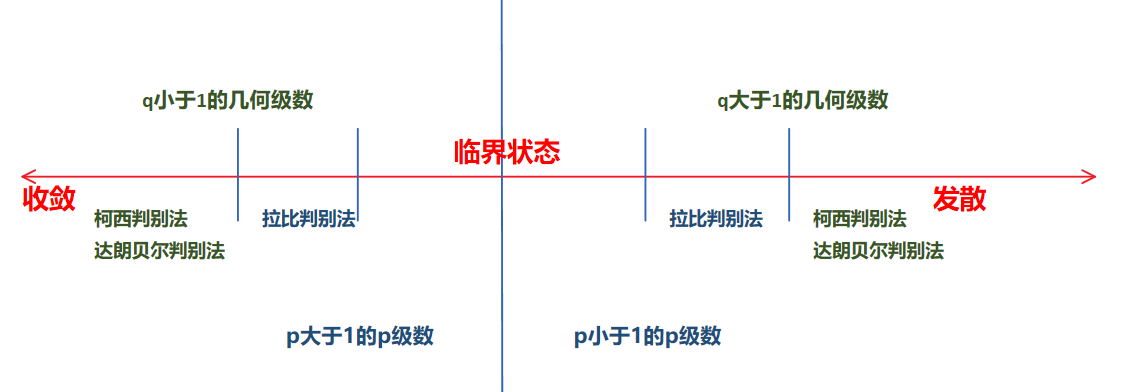
\includegraphics[width=1\linewidth]{收敛.png}
    \caption{不同判别法的有效区间}
    \label{敛散性}
\end{figure}
\par
一些远离临界状态的可以通过和几何级数比较得出结论。靠近临界状态的则要通过和p级数比较得出结论。再靠近临界状态就不能通过和这两者的比较得出结论了。
\subsubsection{和几何级数比}
思路:在极限意义下(n足够大时),把任何一个级数看作几何级数。如果公比q大于1则发散,小于1则收敛。
\[u_n\approx aq^n\]
“抓取”公比q的两种方法:
\begin{enumerate}
    \item 前后作比(达朗贝尔判别法)
\[\lim_{n\to \infty}\frac{u_{n+1}}{u_n}=q \begin{cases}
    q<1:\text{收敛}\\
    q>1:\text{发散}
\end{cases}\]
    \item 开n次根号(柯西判别法)
\[\lim_{n\to \infty}\sqrt[n]{u_n}=q \begin{cases}
    q<1:\text{收敛}\\
    q>1:\text{发散}
\end{cases}\]
\end{enumerate}
\subsubsection{和p级数比}
思路:在极限意义下(n足够大时),把任何一个级数看作p级数。如果p小于1则发散,大于1则收敛。
\[u_n\approx \frac{1}{n^p}\]
“抓取”p的方法(拉比判别法):
\[n\left(\frac{u_n}{u_{n+1}}-1 \right)=n\left( \left(\frac{n+1}{n}\right)^p-1\right)=n((1+\frac{1}{n})^p-1)\approx n(1+\frac{p}{n}-1)=n(\frac{p}{n})=p\]
\[\lim_{n\to \infty}n\left(\frac{u_n}{u_{n+1}}-1 \right)=p\begin{cases}
    p>1:\text{收敛}\\
    p<1:\text{发散}
\end{cases}\]
\section{适用情形}
\begin{enumerate}
    \item 如果知道求和公式可以用定义(部分和)直接判别。
    \item 如果知道原函数可以用无穷积分法判别。
    \item 比几何级数远离临界状态,可以和几何级数比较。(柯西与达朗贝尔)
    \item 比p级数远离临界状态,可以和p级数比较。(拉比)
    \item 也可以通过放缩和其它的级数比较。
\end{enumerate}

\end{document}